%% General definitions
\documentclass{article} %% Determines the general format.
\usepackage{a4wide} %% paper size: A4.
\usepackage[utf8]{inputenc} %% This file is written in UTF-8.
%% Some editors on Windows cannot save files in UTF-8.
%% If there is a problem with special characters not showing up
%% correctly, try switching "utf8" to "latin1" (ISO 8859-1).
\usepackage[T1]{fontenc} %% Format of hte resulting PDF file.
\usepackage{fancyhdr} %% Package to create a header on each page.
\usepackage{lastpage} %% Used for "Page X of Y" in the header.
											%% For this to work, you have to call pdflatex twice.
\usepackage{enumerate} %% Used to change the style of enumerations (see below).

\usepackage{amssymb} %% Definitions for math symbols.
\usepackage{amsmath} %% Definitions for math symbols.
\usepackage{amsthm}
\usepackage{braket}
\usepackage{graphicx}
\usepackage{float}
\usepackage{hyperref}

\usepackage{tikz}  %% Pagacke to create graphics (graphs, automata, etc.)
\usetikzlibrary{automata} %% Tikz library to draw automata
\usetikzlibrary{arrows}   %% Tikz library for nicer arrow heads


%% Left side of header
\lhead{\course\\\semester\\Exercise \homeworkNumber}
%% Right side of header
\rhead{\authorname\\Page \thepage\ of \pageref{LastPage}}
%% Height of header
\usepackage[headheight=36pt]{geometry}
%% Page style that uses the header
\pagestyle{fancy}

\newcommand{\authorname}{Nico Bachmann\\Ruben Hutter}
\newcommand{\semester}{Spring semester 2023}
\newcommand{\course}{Theory of Computer Science}
\newcommand{\homeworkNumber}{6}


\begin{document}

\section*{Exercise \homeworkNumber.1}
We encounter the problem that we want to force an $A$ to be on top of the stack but at the same time not pop $A$.
To work around this, we can add a second transition controlling the $A$.\\
It would look like this:\\\\
1. transition $q_0 \to q_1$:\quad $\epsilon, A \to A$\\
2. transition $q_1 \to q_2$: \quad $c, \epsilon \to B$\\\\
In the first transition we force an $A$ to be on top of the stack by popping it, but then pushing it right back. Then in the second transition we process the $c$ from the input word and add the $B$


\section*{Exercise \homeworkNumber.2}

\begin{enumerate}[(a)]
\item
First we have to introduce two new characters to the alphabet. The $\#$ will be used as delimiter between the different tapes and the $\dot{z}$ where $z \in \Gamma$ is used to save the positions of the different tape-heads on our single tape. With those new characters we can then construct our single tape as follows:
\begin{enumerate}[1.]
\item Move head to the left and write $\#$. (in case it's not allowed to go left, you should shift everything to the right as in 2c) so that you can then write $\#$ all the way to the left.
\item Move head to the right and mark the current character with a dot.
\item Move head to the right until a $\square$ is reached and write $\#$,
\item Move head to the right and write a dotted square: $\dot{\square}$
\item Move head to the right and repeat steps 3 and 4 (k-2)-times.
\item Move head all the way to the left (to the first $\#$)
\end{enumerate}

\item
Here we're scanning from the left-most to the (k+1)st $\#$ to determine what symbols are under virtual heads. To do that:
\begin{enumerate}[1.]
\item Move head to the right until an arbitrary dotted symbol $\dot{z}$ is read.
\item "Go" to that symbols state: $q_{\langle z_1 \rangle}$
\item Repeat step 1 and 2 until the (k+1)st $\#$ is read (end of last tape is reached). The state is now: $q_{\langle z_1, z_2, \dots, z_k \rangle}$
\item Move all the way back to the leftmost symbol.
\end{enumerate}
(Note that it would be more efficient to already process the transitions on the way back instead of going back and then go over the tape a third time.)
\clearpage
\item
We're supposed to write a $\square$ to the right of the current head position. However to the right there is a $\#$ marking the end of that "tape". We now have to right-shift everything from our current position to the end of the tape to make space for the $\square$. To do this:
\begin{enumerate}[1.]
\item Move right (to the $\#$) and replace with a new symbol $\$$ to mark the location where the $\square$ should be put later.
\item Move all the way to the right until the (k+1)st $\#$ is read. (end of tape)
\item Read current arbitrary symbol $z$ move right and write $z$
\item Move left twice
\item Repeat step 3 and 4 until the $\$$ is read.
\item Replace the $\$$ with $\square$ and move right.
\item write $\#$.
\item move left twice.
\end{enumerate}

\end{enumerate}

\clearpage




\section*{Exercise \homeworkNumber.3}

\begin{enumerate}[(a)]
\item
Since Turing-recognizable languages are exactly the type-0 languages (slide B12, page 11), we know that the language $L$ recognized by our given DTM $M$ must be of type-0. However type-0 languages are not closed under complement. Meaning that the complement of a type-0 language does not need to be of type-0.\\
Now since $\bar{L}$ doesn't have to be of type-0, the DTM $M'$ would need to be able to recognize languages that are not type-0. This is not possible!

\item
Let state 1 be the accept state.
Let $M_1$ have only a single transition that goes from state 0 to state 1 by consuming a $0$ and going left.\\
Then let $M_2$ also have only a single transition that goes from state 0 to state 1 by consuming a $1$ but now going right.\\\\
$M_1$ and $M_2$ both accept the word $0$ but are not equal as they go in different directions and are therefore not a "pair".

Our given "product" $M_{1,2}$ then does not include this transition and does not accept $0$. Which contradicts the statement in the question.
\end{enumerate}

\clearpage


\section*{Exercise \homeworkNumber.4}
\begin{enumerate}[(a)]
\item
Encode the rules with the encoding:\\\\

\begin{tabular}{ l | l | l }
states & characters & directions\\
\hline
$ q_0 = bin(0) = 00 $ & $ \square = bin(2) = 10 $ & $ L = bin(0) = 00 $\\
$ q_{accept} = bin(1) = 01 $ & $ 0 = bin(0) = 00 $ & $ R = bin(1) = 01 $\\
$ q_{reject} = bin(2) = 10 $ & $ 1 = bin(1) = 01 $ & \\
\end{tabular}\\\\\\

and we end up with the following:\\\\

\begin{tabular}{ l | l }
rules & \#\# "from" \# "to" \# "read" \# "write" \# "move"\\
\hline
$(q_0 \to q_{accept}) = \square \to \square, L $ & \#\# 0 \# 1 \# 10 \# 10 \# 0\\
$(q_0 \to q_{reject}) = 0 \to 1, R $ & \#\# 0 \# 10 \# 0 \# 1 \# 1\\
$(q_0 \to q_{reject}) = 1 \to 0, L $ & \#\# 0 \# 10 \# 1 \# 0 \# 0\\\\
\end{tabular}\\\\\\ 

Now we transform our new words (rules) over \{0, 1\} with the mapping:\\
$0 \to 00 \qquad \qquad 1 \to 01 \qquad \qquad \# \to 11$\\\\
to:\\
1111 00 11 01 11 0100 11 0100 11 00\\
1111 00 11 0100 11 00 11 01 11 01\\
1111 00 11 0100 11 01 11 00 11 00\\\\

and then chain them together in an arbitrary order:\\
11110011011101001101001100 111100110100110011011101 111100110100110111001100\\
and have successfully encoded the given Turing machine in a word over \{0, 1\}.

\clearpage

\item
To decode $w$ we have to reverse the steps from (a).

\begin{enumerate}[1.]
\item split at the $\#\#$ and $\#$ separator encoded as 1111 or 11:\\\\
1111 00 11 00 11 00 11 00 11 01 \\
1111 00 11 01 11 01 11 01 11 01 \\
1111 00 11 0100 11 0100 11 00 11 01 \\

\item decode the character pairs back to their integer values:\\\\
\#\# 0 \# 0 \# 0 \# 0 \# 1 \\
\#\# 0 \# 1 \# 1 \# 1 \# 1 \\
\#\# 0 \# 10 \# 10 \# 0 \# 1 \\

\item decode the integer values back to their characters:\\\\
$q_0 \to q_0 = 0 \to 0, R$\\
$q_0 \to q_{accept} = 1 \to 1, R$\\
$q_0 \to q_{reject} = \square \to \square, R$\\\\

\begin{figure}[H]
		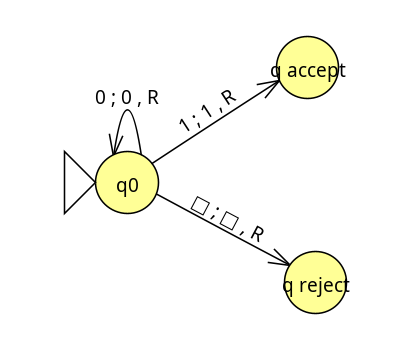
\includegraphics[scale=0.45]{ex4b.png}
		\centering
\end{figure}

\end{enumerate}
\end{enumerate}

\section*{Exercise \homeworkNumber.5}
\begin{enumerate}
\item False because a language $L$ is Turing-decidable, iff both $L$ and $\bar{L}$ are Turing-recognizable. However type-2 languages are not closed under complement so $\bar{L}$ does not have to be of type-2 and therefore also doesn't have to be Turing-recognizable. And if that's the case, $L$ is not Turing-decidable which contradicts the given statement.

\item True because if a language $L$ is Turing-decidable, $L$ and $\bar{L}$ both have to be Turing-recognizable and therefore be of type-0. And because they have to be type-0, they also need to have a grammar.
\end{enumerate}

\end{document}
